\documentclass[12pt]{article}
\usepackage[utf8]{inputenc}
\usepackage[russian]{babel}
\usepackage{graphicx}
\usepackage{amsmath}
\graphicspath{ {./images/} }


\begin{document}

Дубровских Никита 221-361

\textit{\textbf{Вариант 7}}

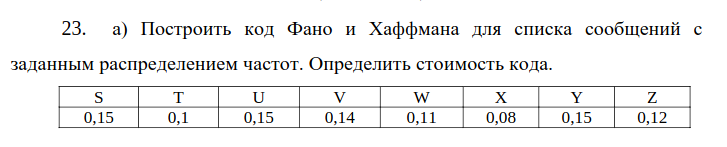
\includegraphics[scale=.5]{23.png}

Проверим выполнимость необходимого условия:

0,15 + 0,1 + 0,15 + 0,14 + 0,11 + 0,08 + 0,15 + 0,12 = 1

Расположим элементы в порядке убывания вероятностей. Затем будем
последовательно делить, не меняя порядка, все элементы на две группы,
максимально близкие по суммарной вероятности (т.е. модуль разности сумм
вероятностей первой и второй группы должен быть минимальных из всех
возможных разбиений на группы). Для «верхней» группы будем ставить
значение 0, «нижней» - 1:

\begin{center}
	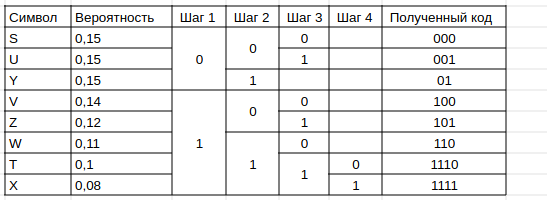
\includegraphics[scale=.75]{23_2.png}
\end{center}

Найдем стоимость кода (средняя длина кодового слова). Он является
критерием степени оптимальности кодирования. Вычислим ее в нашем случае.

$$l=\sum_{i=1}^8l_i \cdot p_i = 3 \cdot (0,15 \cdot 2 + 0,14 + 0,12 + 0,11) + 2 \cdot 0,15 + 4 \cdot (0,1 + 0,08) = $$

$$=3 \cdot 0,67 + 0.3 + 4 \cdot 0,18 = 2,01 + 0,3 + 0,72 = 3,03$$

По Хаффману:




\end{document}
